\chapter{Modelling the deformation of hollow objects in real-time}
\label{chap7}
\begin{shortAbstract}
A short abstract for the upcoming chapter
\end{shortAbstract}


\section{Introduction: the problematic}
The human body is composed of various deformable anatomical structures. A key challenge of soft-tissue modelling is the variousness of the mechanical behaviours. The shape and the internal structure may be very different from one organ to another. If you take the liver for instance, it is a solid organ composed of four lobes, each one made up of units called lobules. Each lobule consists of a central vein surrounded by liver cells and constitutes the end of a dense network of blood vessels. This particular internal structure has a strong influence on the mechanical properties of the liver. In contrast, the colon is a long and hollow organ. It consists of four sections which all have different shapes and material properties. Consequently, it seems unrealistic to use a unique model for all tissues. Yet, most of previous works focus on volumetric models that are able to capture the behaviour of solid organs. In fact in the field of medical simulation, very few models have been proposed for simulating, in real-time, the deformation of thin anatomical structures whose volume is negligible compared to their surface area. Examples include hollow structures, such as the wall of blood vessels, or membranes, such as the Glisson?s capsule surrounding the liver. It is also of particular interest to us for modelling the colon in our colonoscopy simulator and for simulating the deployment of the implant in cataract surgery. 

Numerous models are available in the literature to describe physics of thin objects, from fairly simple and naive approaches to more complex and thorough representations. Continuum mechanics provides many formulations able to accurately describe stresses occurring within thin objects. Most of them fall into one of the following two categories: plate theory or shell theory. Those theories have been a subject of interest in the mechanical community for decades. The difference between these two kinds of structures is very well explained by \cite{Liu03} and can be summarised by the fact that plate bending elements can only carry transversal loads while shells can undergo more complex deformations. 
For instance, if we consider the horizontal board of a bookshelf, that board can be approximated as a plate structure and the transversal loads are the weight of the books. A typical deformation of the board is illustrated in \fig{chap7:fig-boards} (a). Conversely, a shell structure can carry loads in all directions, and therefore can undergo bending, twisting and in-plane deformation (see \fig{chap7:fig-boards} (b)). 
%
\begin{figure}[ht]
\centering 
\subfloat[Plate theory]{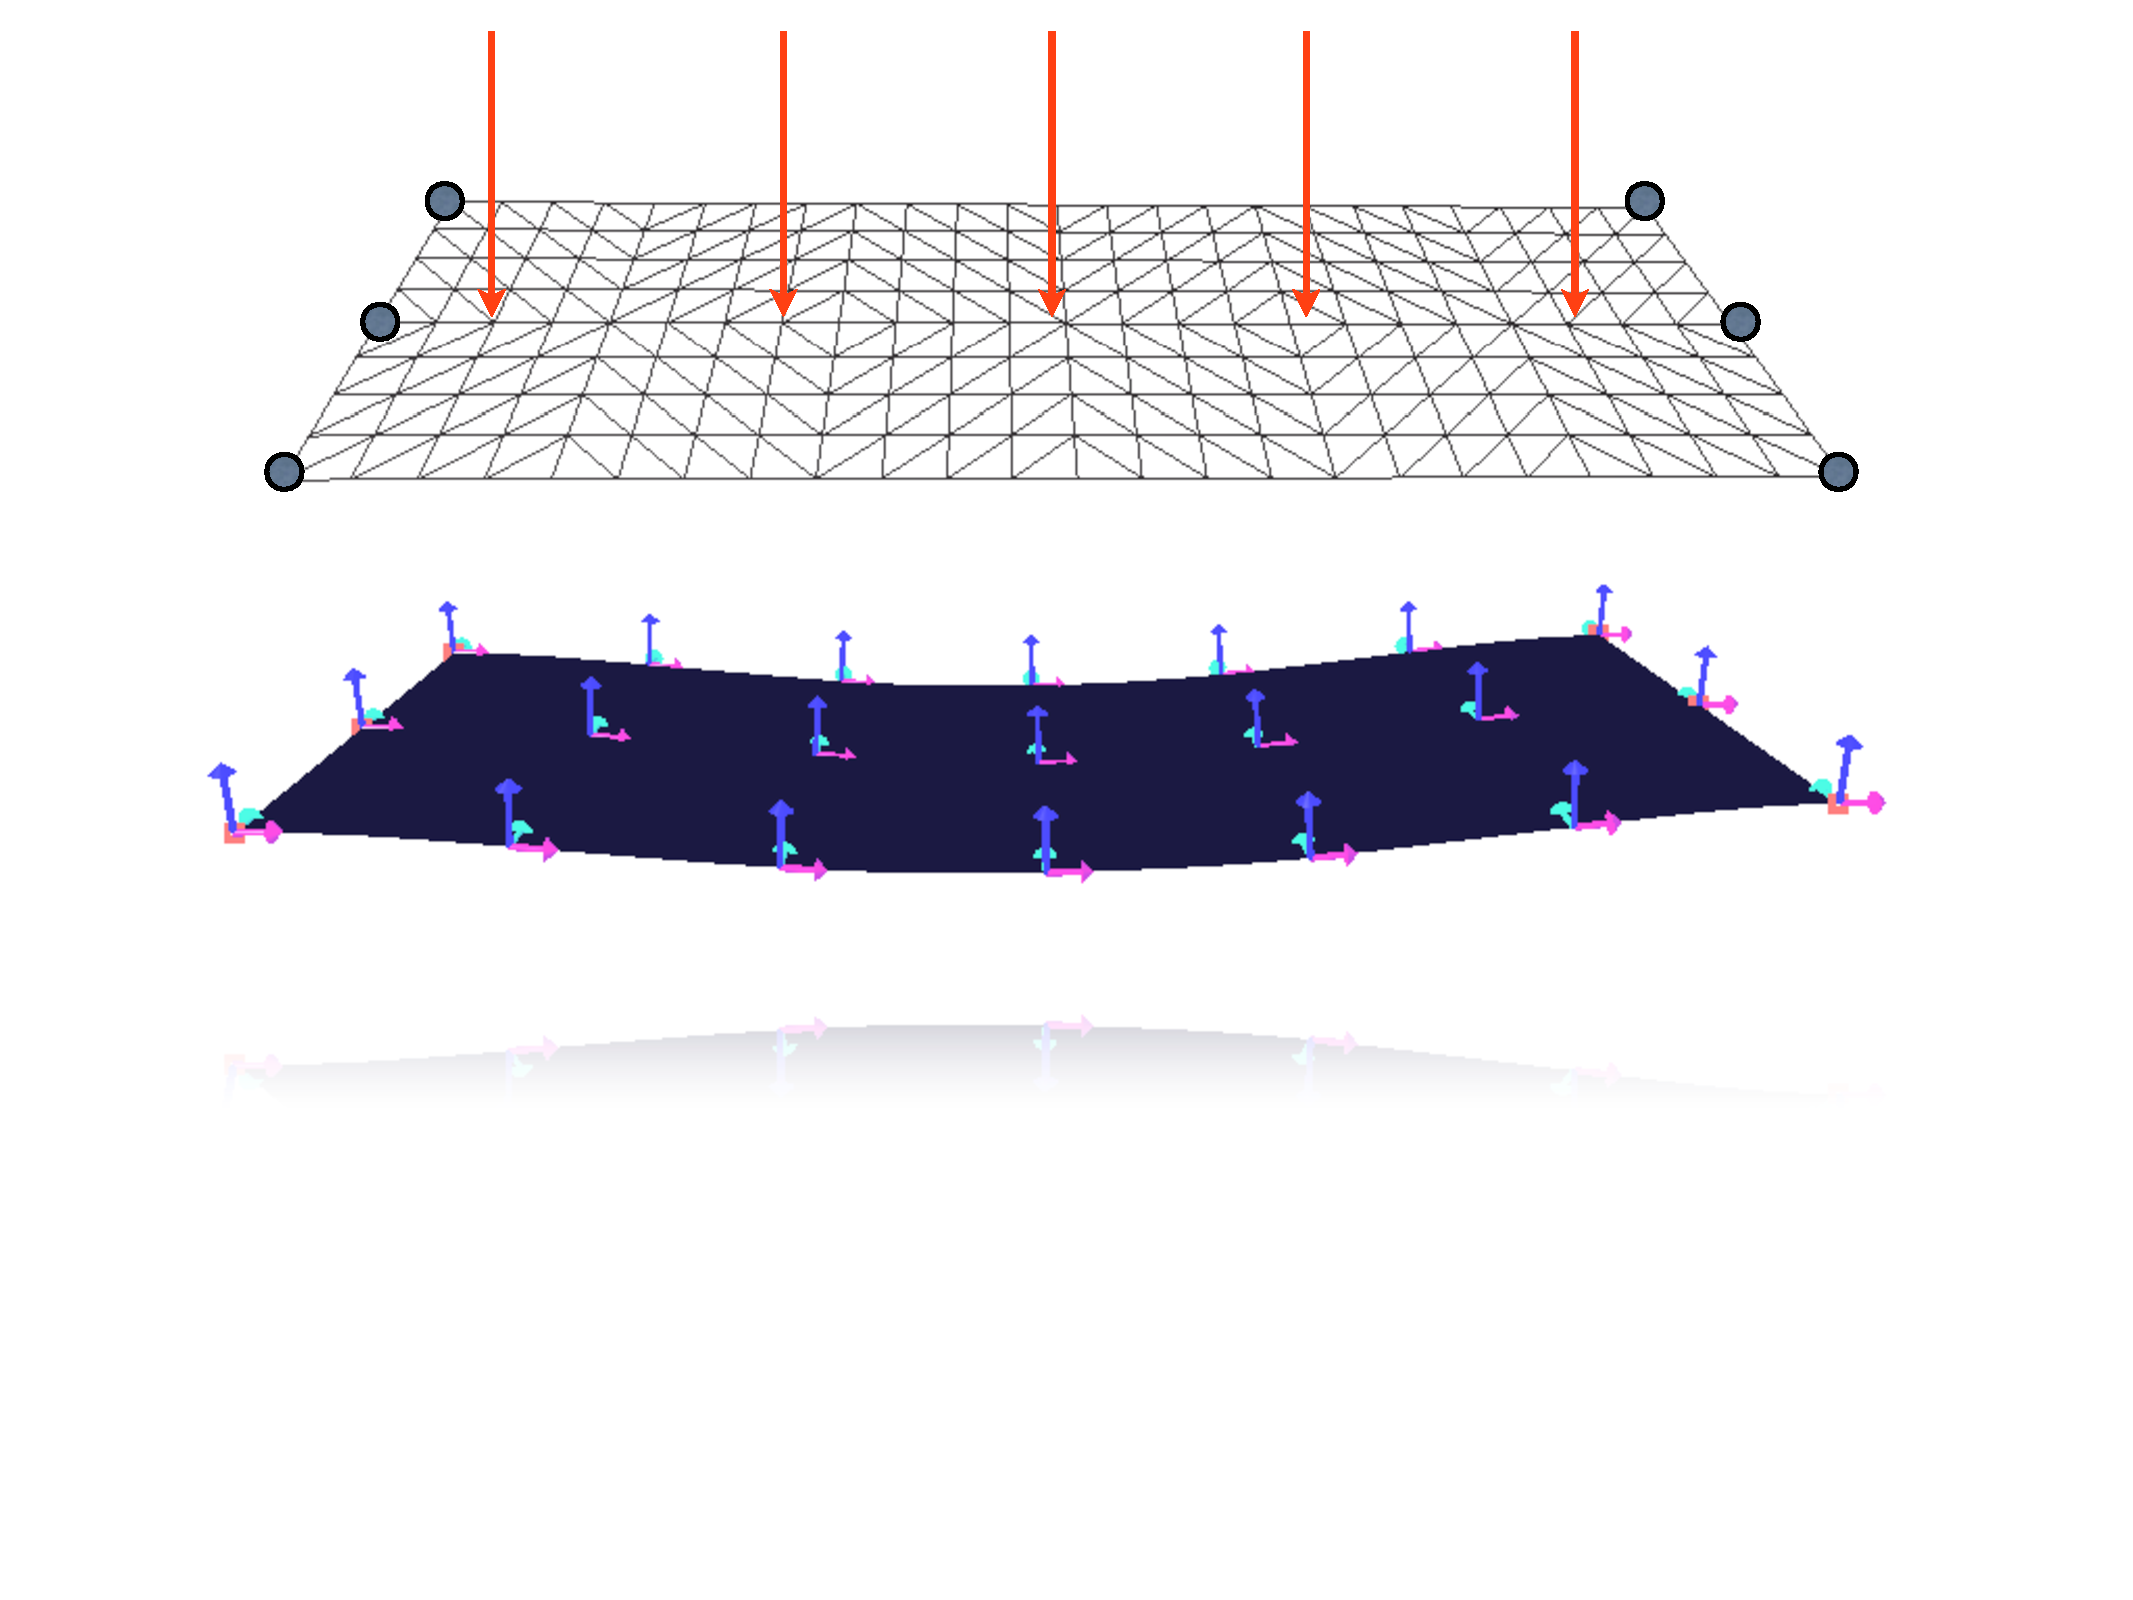
\includegraphics[width=6.5cm]{chapter7/board_bending.pdf}}
\hfill 
\subfloat[Shell theory]{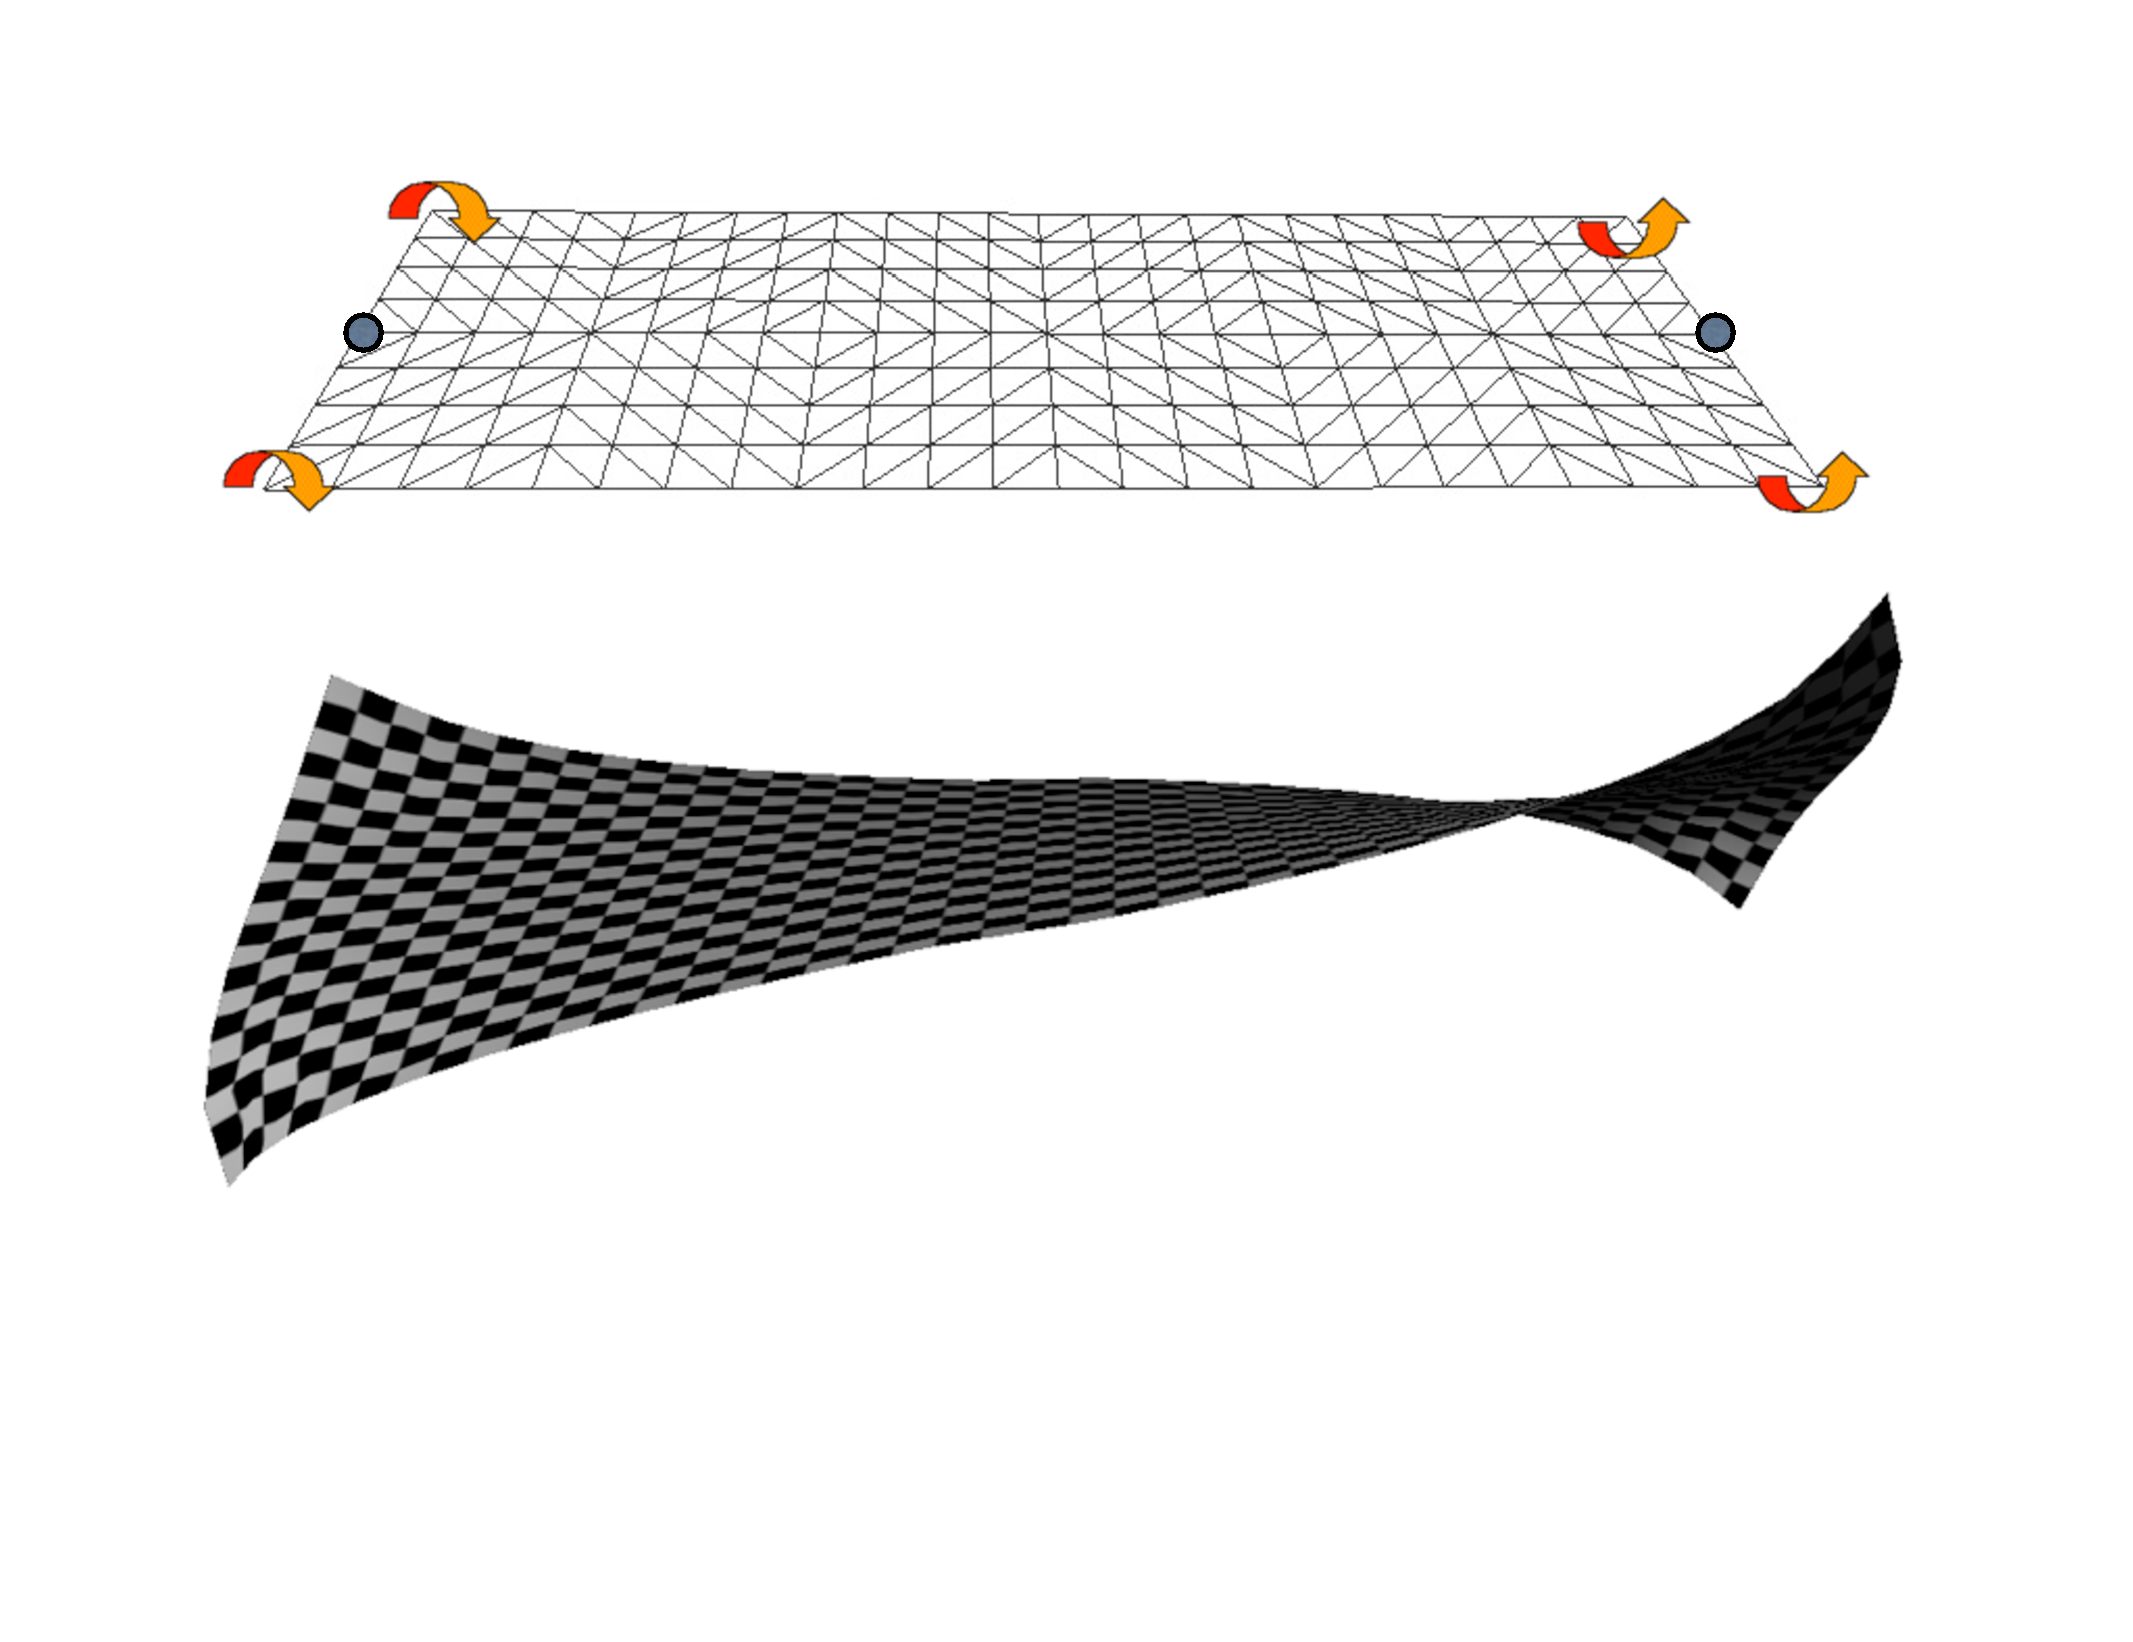
\includegraphics[width=6.5cm]{chapter7/board_twist.pdf}}
\caption[Illustration of the key difference between plate and shell theory]{Illustration of a key difference between various models of thin objects. While thin plate theory allows to describe bending (a), it cannot represent more complex deformations such as twist (b) which is captured by shell theory.}
\label{chap7:fig-boards}
\end{figure}


Development of a satisfactory physical model that runs in real-time but produces visually convincing animation of thin objects has been a challenge in Computer Graphics, particularly in the area of cloth modelling. Rather than resorting to shell theory which involves the most complex formulations in continuum mechanics, most of works have relied on discrete formulations. We will first discuss early approaches based on mass-spring models. Then we will present techniques relying on the derivation of a bending energy from geometric considerations. At last, we will introduce approaches based on shell theory using the more computationaly demanding finite element method.

%	\subsection{Colonoscopy simulator project: needs for colon}
%	\subsection{Cataract surgery, stenosis: other needs for implants/blood vessels}
		
\section{Mass-spring models}

Early approaches to thin objects modelling only considered in-plane deformation, and often relied on mass-spring models. This technique was already presented in section \ref{chap4:massSprings} so we only present their use for modelling thin structures. \cite{Provot95} improved a mass-spring model to take into account the non-elastic properties of woven fabrics. Because of the high stiffness of textiles, mass-spring models are particulary unstable when used to simulate cloth. The author proposed a new method inspired from dynamic inverse procedure. Under certain conditions and because of the linear law employed in a mass-spring system, the fabrics may become super-elastic. \citeauthor{Provot95} suggested to set a threshold on the deformation rate to correct this super-elasticity (see \fig{chap7:fig-sheet}). 
%
\begin{figure}[ht]
\centering 
\subfloat[Initial position]{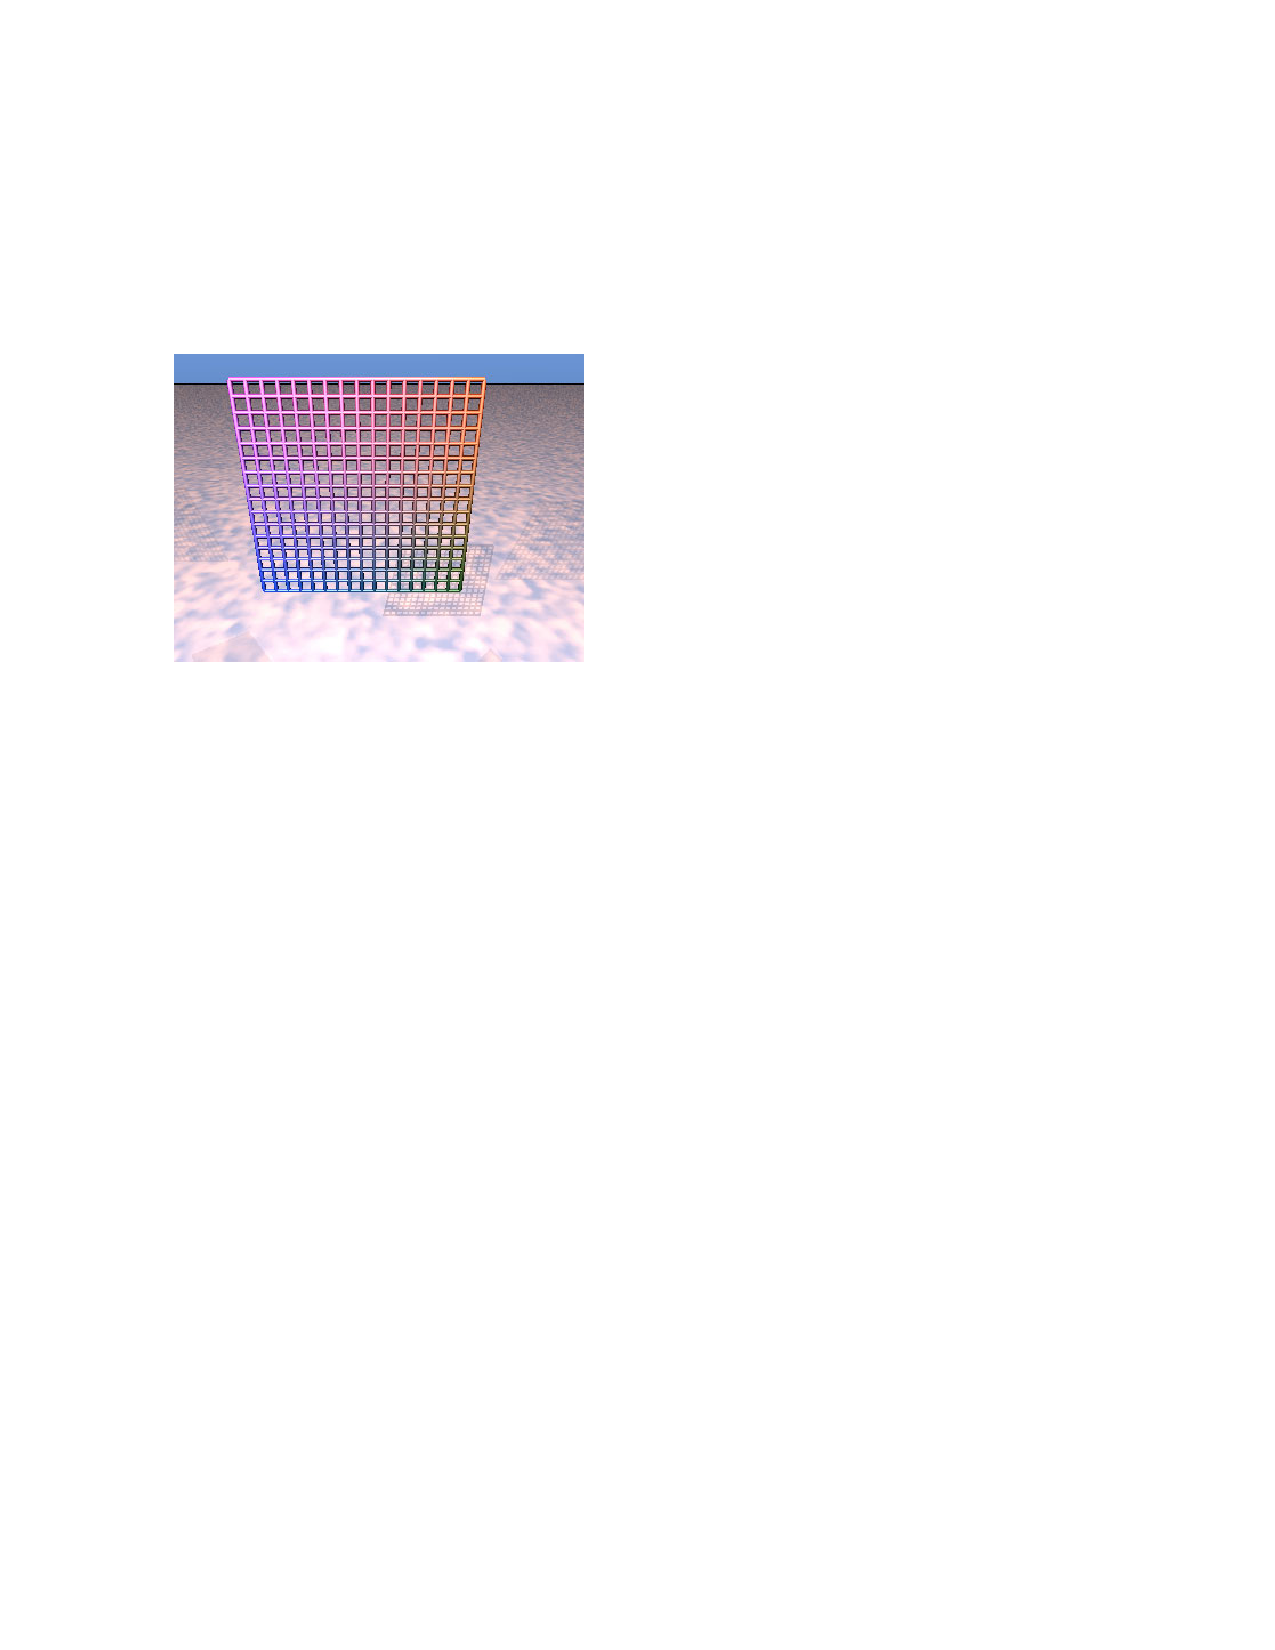
\includegraphics[width=4.5cm]{chapter7/sheet1.pdf}}
\hfill 
\subfloat[Uncorrected]{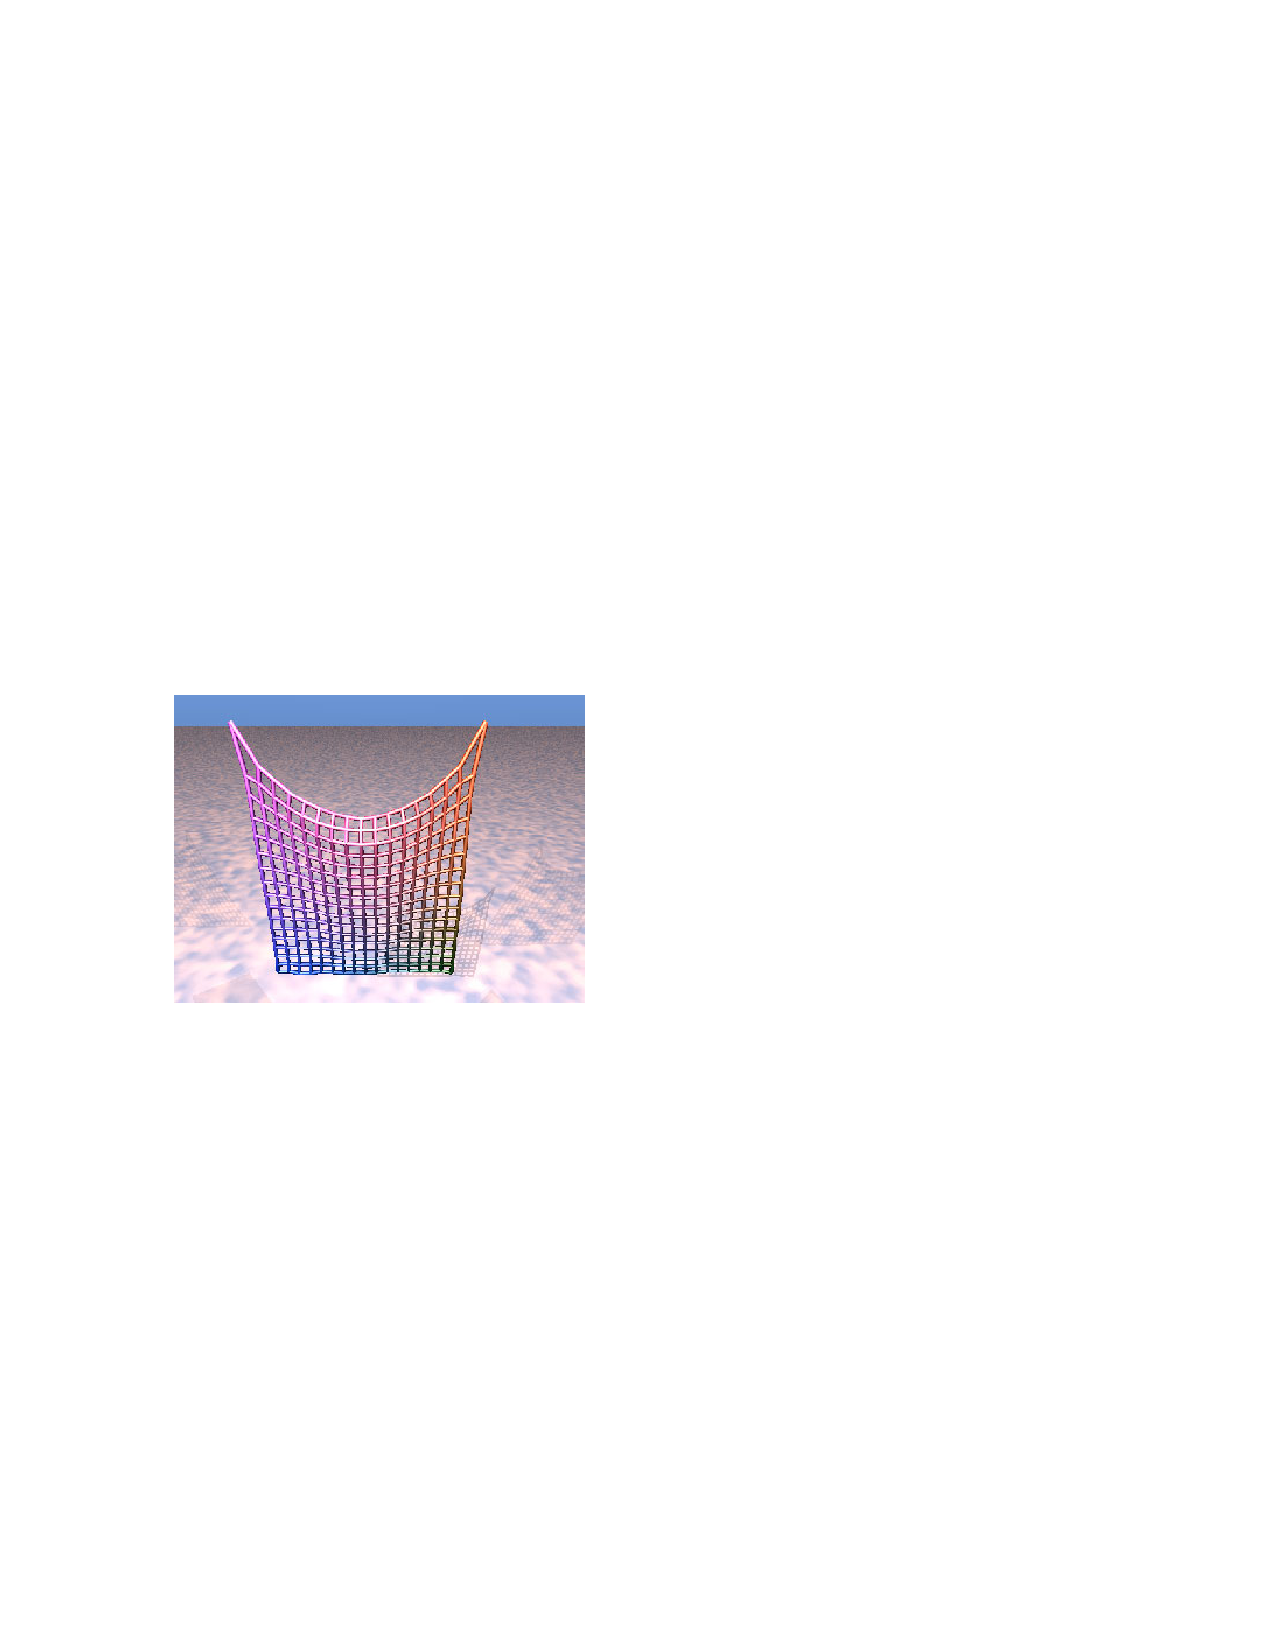
\includegraphics[width=4.5cm]{chapter7/sheet2.pdf}}
\hfill 
\subfloat[Corrected]{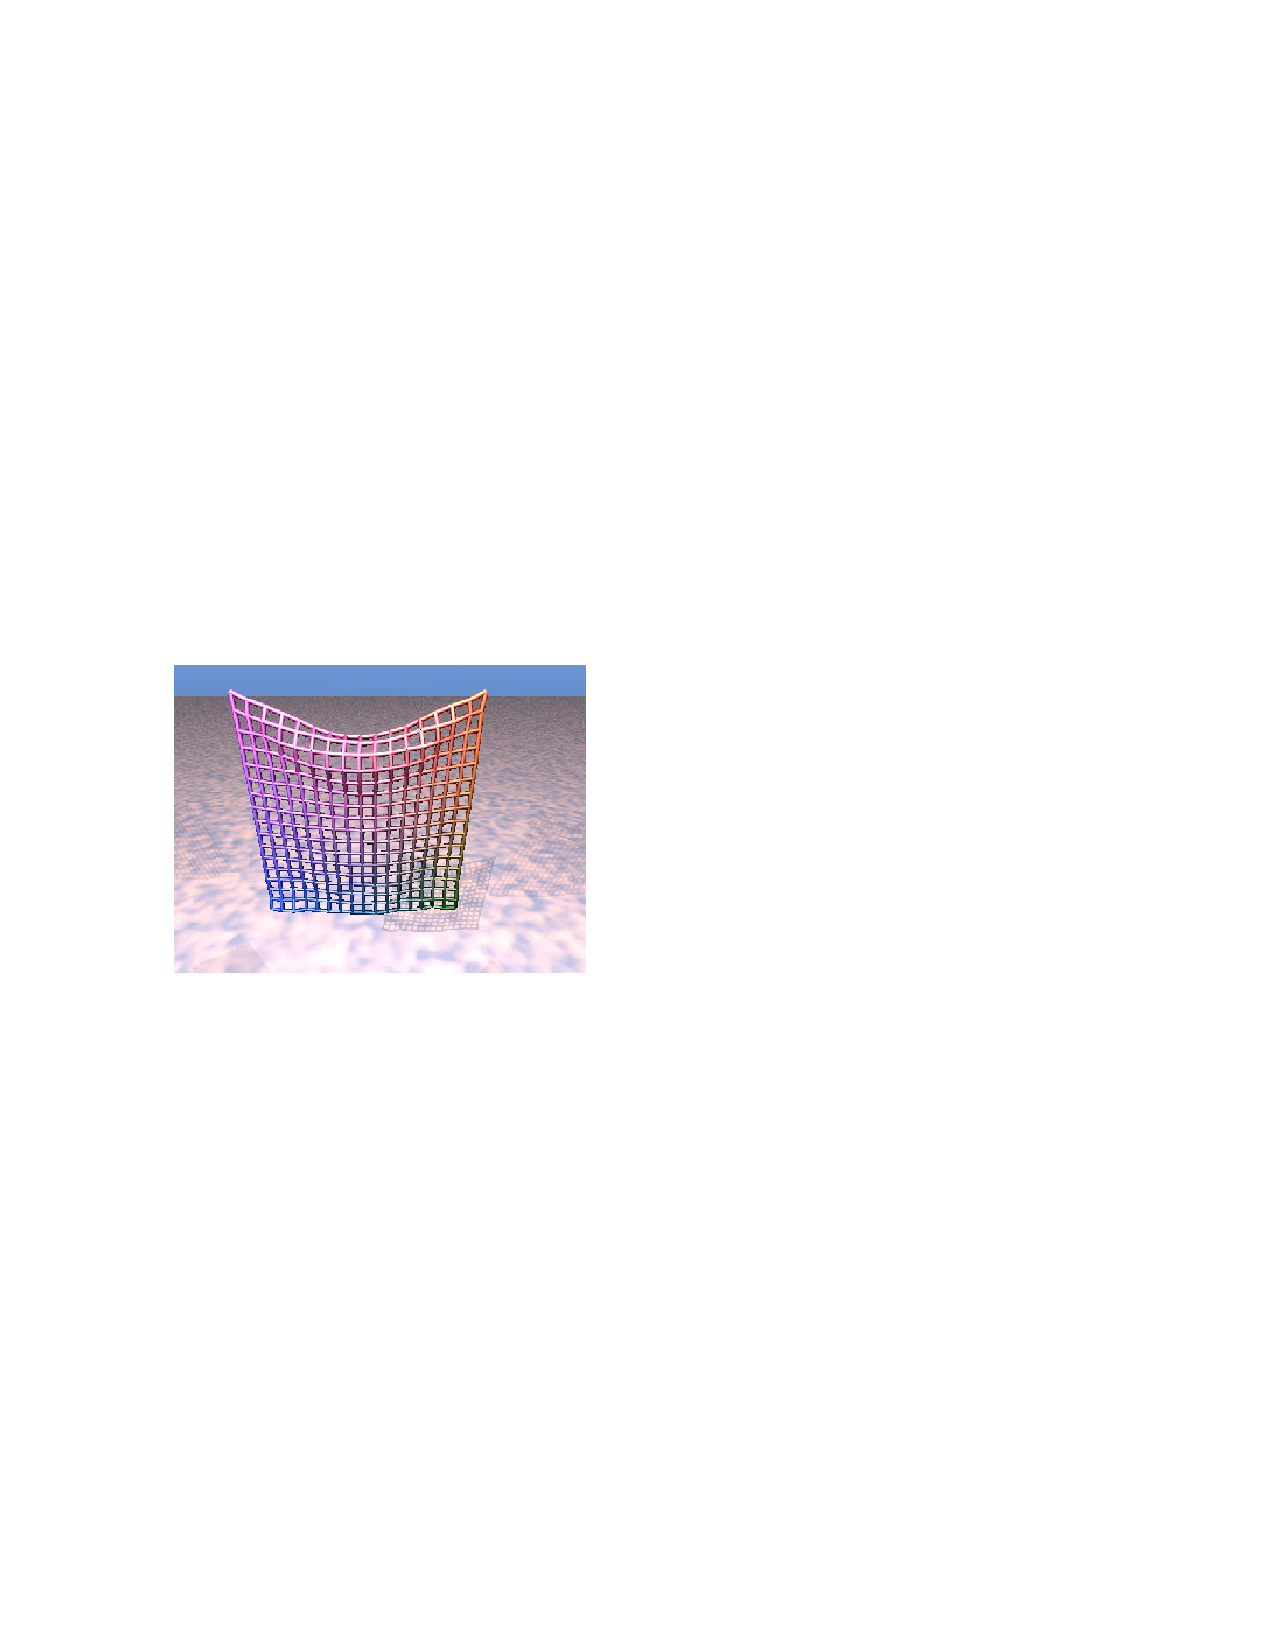
\includegraphics[width=4.5cm]{chapter7/sheet3.pdf}}
\caption{Deformation of a sheet hanging by two adjacent corners. Images courtesy of \cite{Provot95}.}
\label{chap7:fig-sheet}
\end{figure}

To improve the computational efficiency, \cite{Hutchinson96} presented a mechanism for adaptively refining the network of mass-springs to concentrate efforts only where it is needed. When potential inaccuracies are detected, the object is locally refined in the affected region, and the simulation may carry on. \cite{Oshita01} used a sparse triangular mesh and an interpolation to generate a dense mesh. 

A limitation of mass-spring models that we often hear is the difficulty to derive spring stiffness from elastic properties (Young's modulus and Poisson's ratio). With this drawback in mind, \cite{Volino97} improved a mass-spring system by allowing the modelisation of Young's modulus and Poisson's ratio (see \fig{chap7:fig-fabricSquares}). They also added a correction technique relying on the control of damping and velocities to ensure the stability of their model. 
%
\begin{figure}[ht]
\begin{center}
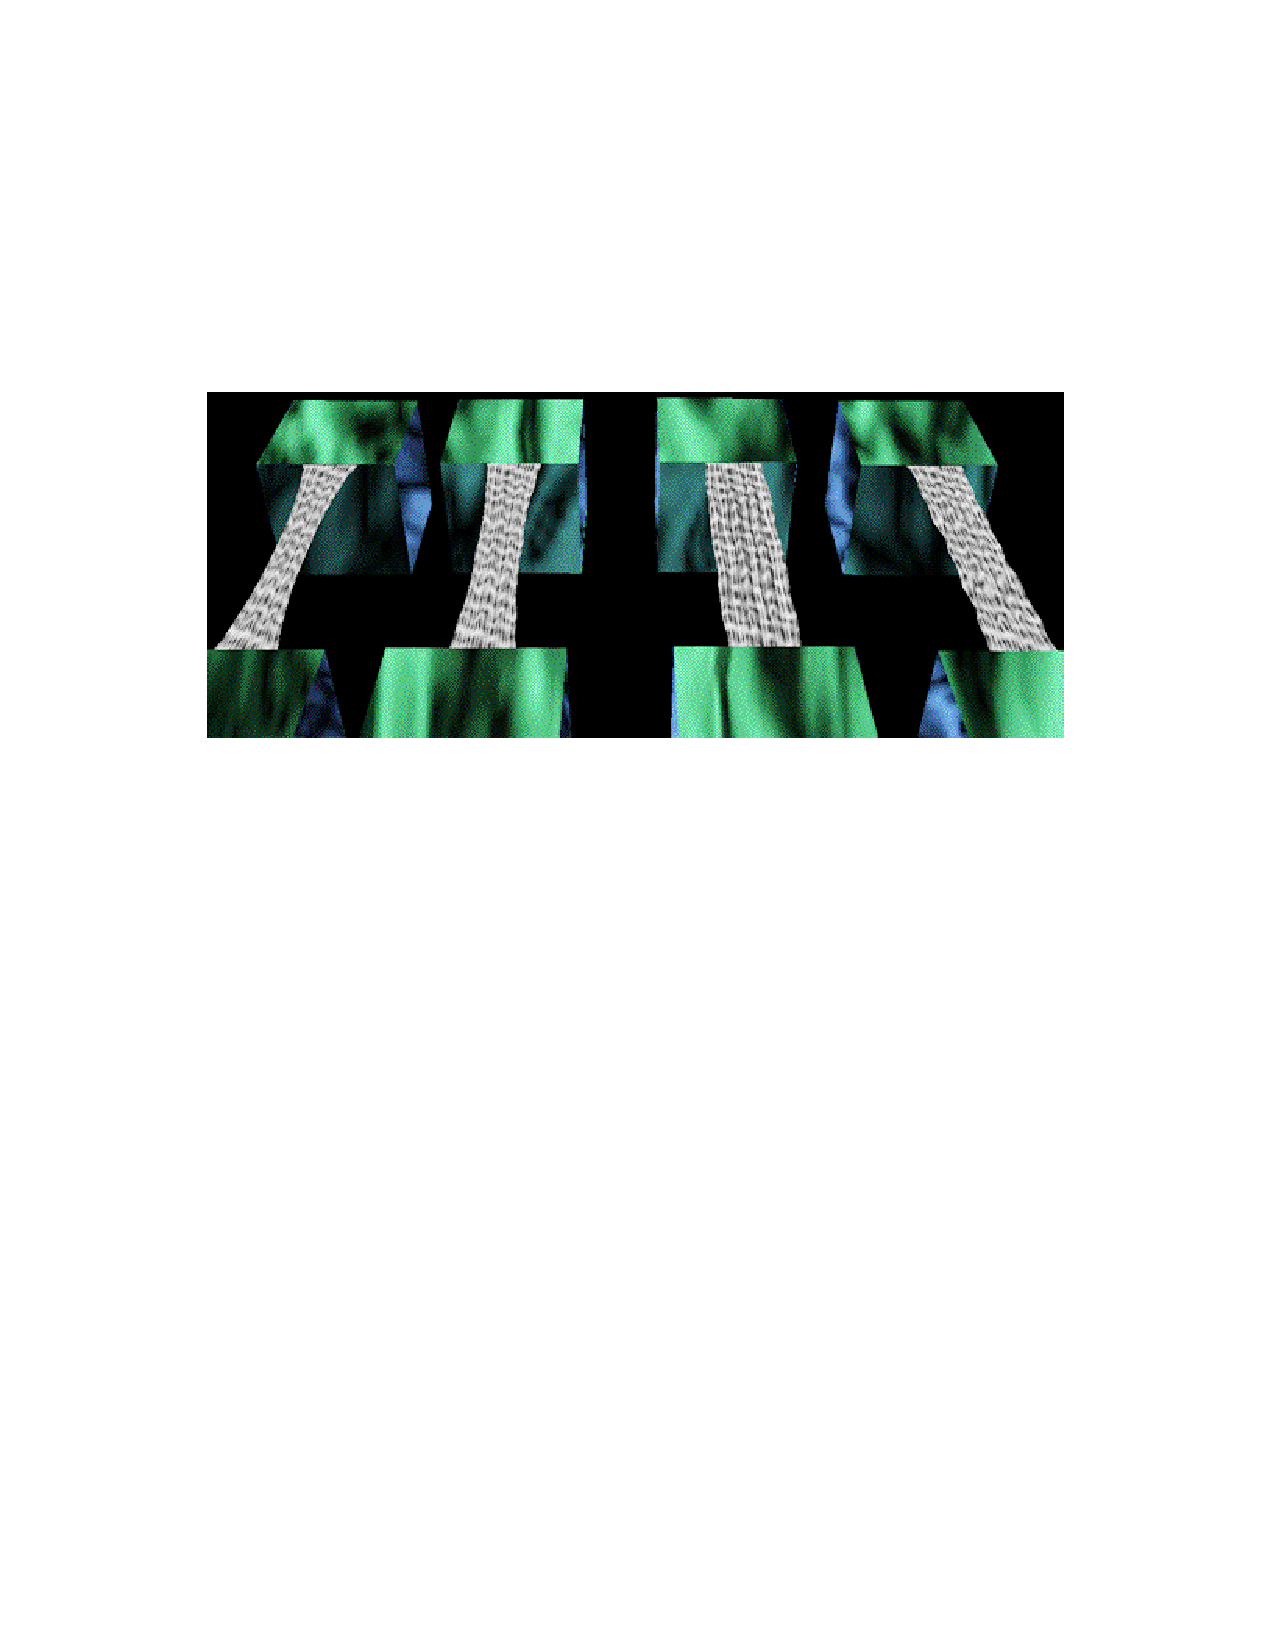
\includegraphics[width=12cm]{chapter7/fabricSquares.pdf}
\caption[A $400\,$\% stretched fabric square]{A $400\,$\% stretched fabric square with various Poisson's ratio.}
\label{chap7:fig-fabricSquares}
\end{center}
\end{figure}

Other works have considered adding bending through angular springs. For instance, \cite{Taskiran05} have chosen to use a linear representation of angular springs to supply bending and torsion effects in hair modelling, which allowed them to simulate curly hair with good realism. All the forces related to springs were implemented: gravity, repulsions from collision, absorption, friction, etc. They could simulate up to a few hundreds of hair stripes in real-time. \cite{Wang07} successfully used a network of linear and angular springs to describe bending and twisting of catheters and guidewires in an interventional radiology simulator. 

More recently and in the field of medical simulation, \cite{Hammer08} employed a mass-spring model to simulate the mitral valve closure for surgical planning. In their model, triangle sides are treated as linear springs and sides shared by two triangles are treated as bending springs. 

	
\section{Techniques relying on the derivation of a bending energy}

Another kind of approach is to geometrically derive a bending energy. For instance, \cite{Baraff98} derived stretch, bending and shear energies geometrically. They also used an adaptative time stepping based on detection of large stretches. Using an implicit integration allows the authors to use large time steps and substantially increase the stiffness with a limited impact on performance. 


%Among the different models introduced recently we can mention the work of \cite{Choi07} and \cite{Bridson03}. \citeauthor{Choi07}  proposed a real-time simulation technique for thin shells undergoing large deformations. The authors adopt the energy functions from the discrete shells proposed by \cite{Grinspun03}. For real-time integration of the governing equation, they adapted a modal analysis technique, called modal warping. The resulting simulations run in real-time even for large meshes, and the model can handle large bending and/or twisting deformations with acceptable realism. \citeauthor{Bridson03} followed the same energy approach to derive their bending model but improved the resolution of the equations by suggesting a novel mixed implicit/explicit integration scheme. They also presented a post-processing method for treating cloth-character collisions that preserves folds and wrinkles. \cite{Pabst08} improved the bending modelling used by \citeauthor{Bridson03} to allow the integration of measured material data. 
%
%A method to use thin shell dynamics with point sampled surfaces for efficient animation was recently proposed by \cite{Wicke05} where the curvature of the shell is measured through the use of fibers.		
		
		
		
\section{Techniques based on continuum mechanics}

% Co-rotational methods
% More recently, \cite{Allard09} modelled the membrane of the lens capsule with a co-rotational finite element formulation in a cataract surgery simulator. The goal was to simulate the anisotropic fracture progation
